\section{Avionics In-Flight Event Overview} \label{section:avionics-appendix}

\subsection*{Flight Mode}
The computer will track changes through the following phases of flight. Each phase will be represented in a Stateflow model. These states and their transitions may change slightly as the design of the vehicle chages over time.

\subsubsection*{On the Pad}
This phase happens when the computer is powered on and the rocket is vertical on the rail. All sensor calibrations should happen during this phase. During this phase the computer will be checking the accelerometer data to check for liftoff, but not recording the data yet. 

\subsubsection*{First Stage Burn}
One liftoff is detected by the accelerometer the computer enters the first stage burn phase. During this phase it is measuring and recording acceleration data at the highest frequency possible. It will also be measuring and recording data from all other sensors, and sending it the state estimation algorithm. Additionally, the first stage lockout countdown begins as soon as the rocket enters this phase. No events (eg. stage separation/ignition/parachutes) can be triggered until the first stage lockout countdown has reached 0. 

\subsubsection*{Combined Coast/Staging}
After the primary motor has burned out and the first stage lockout has ended, the computer will enter the staging phase. 

\noindent\textbf{Hot Separation:} If a ``hot separation'' method is used, the rocket will separate stages by igniting the second stage motor while the two stages are still together. This could be used in combination with/as a backup to drag separation. 

\noindent\textbf{Passive (Drag) Separation:} If a passive separation method is used, the two stages will not be held together. They may naturally separate after first stage burnout, due to drag on the first stage. This method may include a separation detection circuit. If this does not naturally occur, a hot separation will occur, assuming the conditions are still met.

\noindent\textbf{Active Separation:} If an active staging method is used, a mechanism will hold the stages together until commanded to separate. We do not expect to use this method.

\subsubsection*{Second Stage Ignition}
Second stage ignition can only occur if the following conditions are met:

\begin{itemize}
    \item Rocket is above a certain altitude
    \item Rocket is not tilted more than a certain threshold from vertical
    \item Stage separation has been triggered (if applicable)
    \item A set time delay since stage separation has passed (if applicable)
\end{itemize}

If all these conditions are met, second stage ignition will occur. If they are not met, the computer will skip to the apogee detection phase without igniting the second stage. 

\subsubsection*{Second Motor Burn}
The computer enters this phase upon detection of the second stage igniting (from accelerometer data). Upon entering this phase the second stage lockout countdown will start. If ignition is not detected within a certain number of seconds after it should have happened, the computer will skip to the apogee detection phase, without starting the timer.

\subsubsection*{Coast/Apogee Detection}
In this phase, the computer will use data from the state estimation to detect when the rocket has passed apogee. 

\subsubsection*{Drogue Deploy/Descent}
After apogee has been passed and any active lockout timers have ended, the drogue chute will deploy.

\subsubsection*{Main Deploy/Descent}
Once data from the state estimation function shows that the rocket is under the main deployment altitude, the main chute will be deployed. 

\subsubsection*{Touchdown}
Once the rocket is on the ground stop, it will stop recording data, safe itself, and shut down.

\subsection*{Flowchart of Phases}
The state flow diagram is shown in \Cref{figure:avionics-stateflow}. Each rounded box is a flight phase (Stateflow state). The phase will help the State Estimation determine which prediction model to use. Each parallelogram box is an event that needs to be triggered. These could be their own states or just happen upon entering/exiting the previous/next state. The circles show different options that depend on the rocket configuration (stage and separation method). See \Cref{table:av-state-transitions} for transition criteria for each arrow. In the table, yet-undetermined parameters are left as ``BLANK''.

\begin{figure}[htbp]
    \centering
    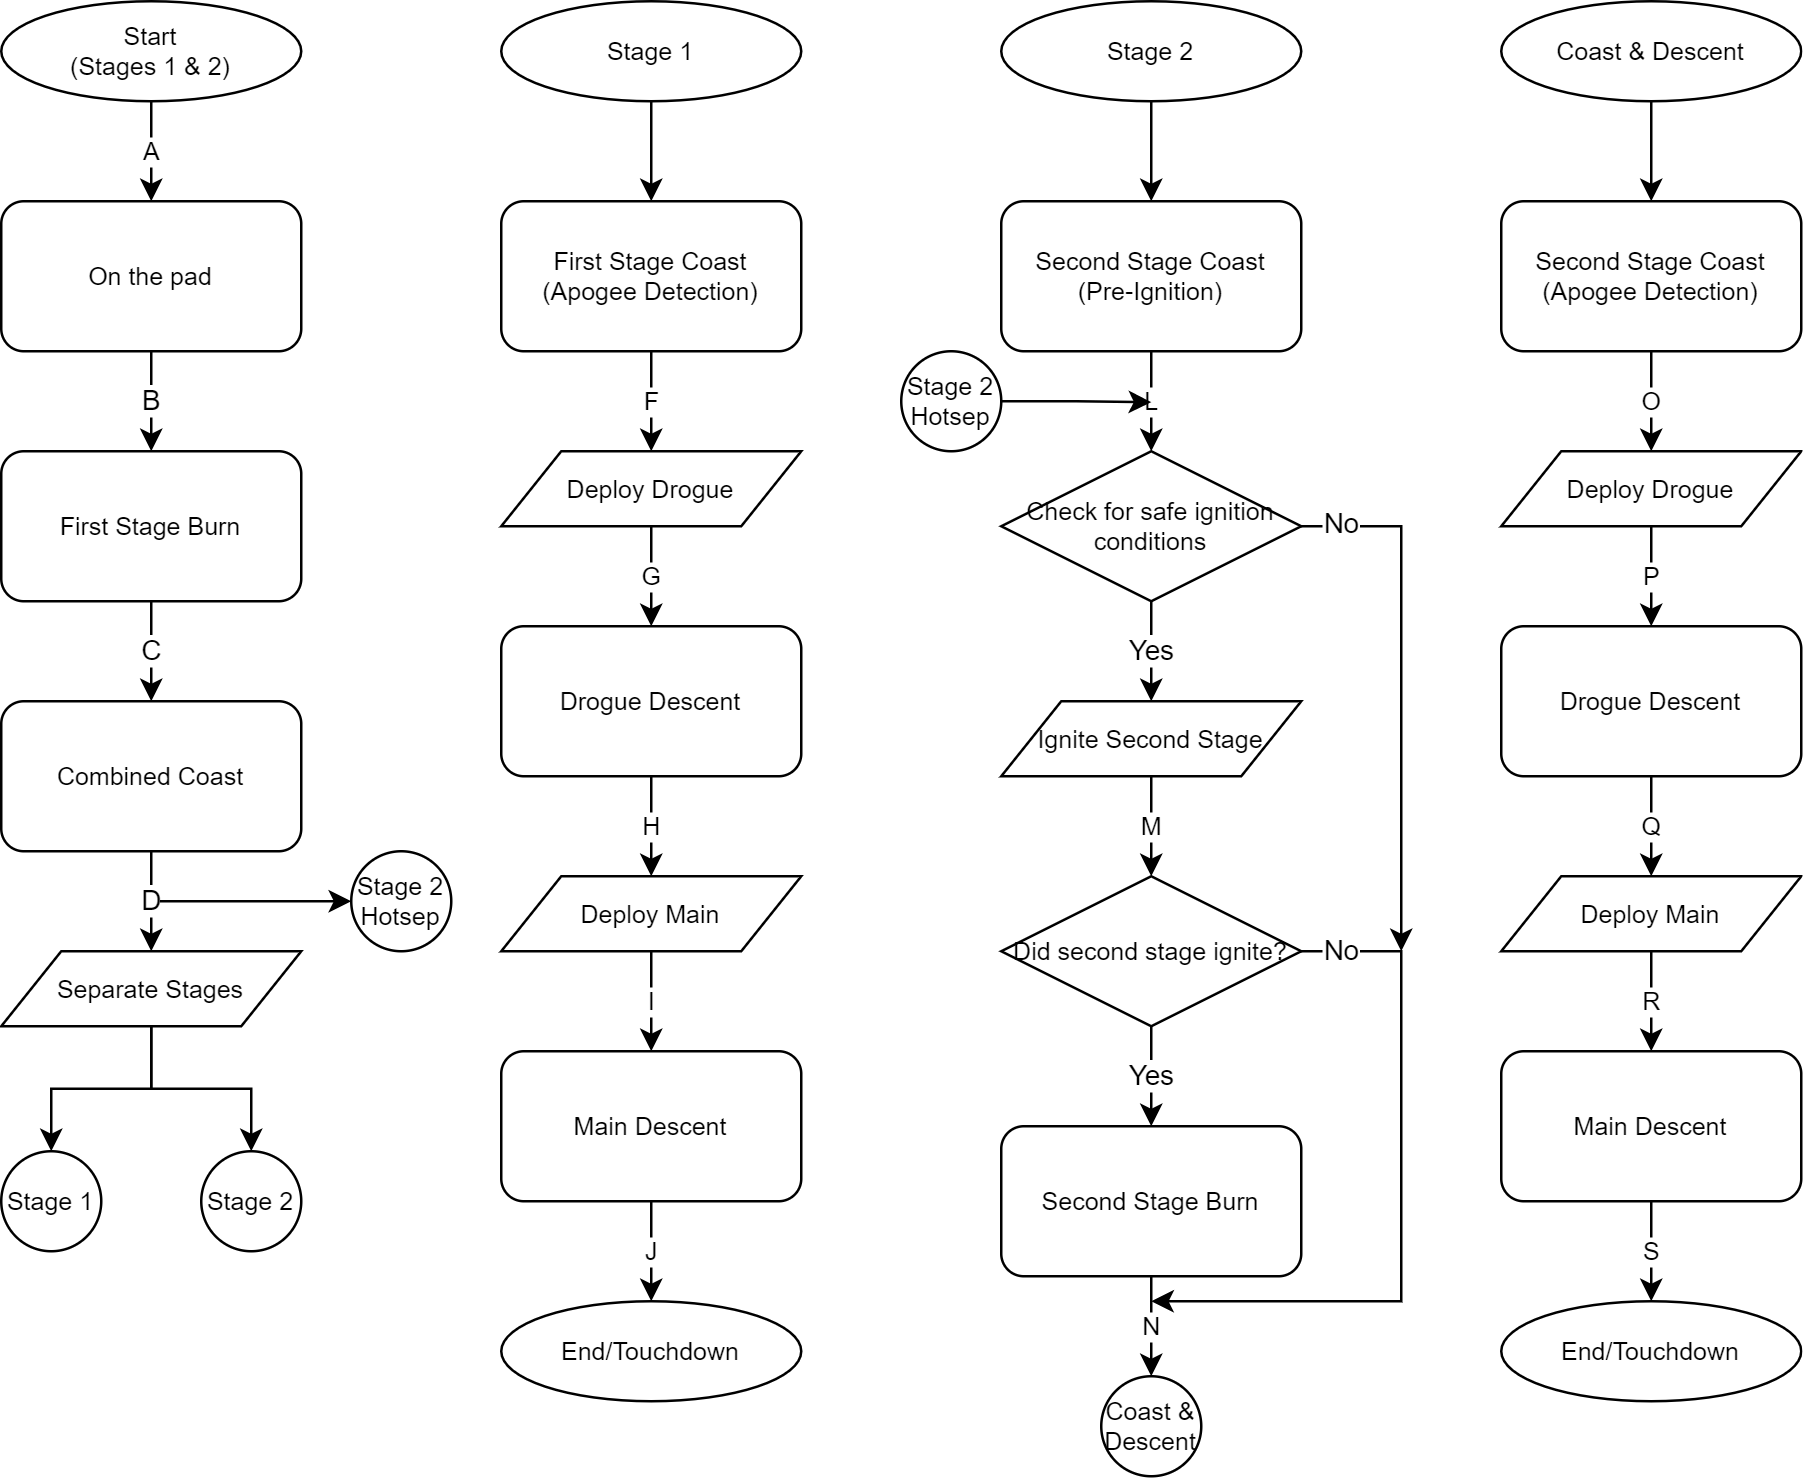
\includegraphics[width=\textwidth]{images/avionics-stateflow}
    \caption{The preliminary avionics flight event logic stage flow diagram}
    \label{figure:avionics-stateflow}
\end{figure}

\begin{table}
    \centering
    \small
    \setlength{\offset}{\baselineskip}
    \begin{longtable}{>{\raggedright\arraybackslash}p{1.5cm} >{\raggedright\arraybackslash}p{10cm} >{\raggedright\arraybackslash}p{3cm}}
        \toprule
            \textbf{Transition Label} & \textbf{Criteria} & \textbf{Transitions To} \\
        \midrule
            A & The rocket is vertical on the launch rail. This means the pitch angle is 90 \(\pm\) BLANK degrees. & On the Pad \\
            B & The accelerometer detects positive acceleration in the vertical direction greater than BLANK m/s\(^2\) for longer than BLANK milliseconds. & First Stage Burn \\
            C & After first stage burnout: The accelerometer detects acceleration in the vertical direction less than BLANK m/s\(^2\) for longer than BLANK milliseconds. & Combined Coast \\
            D & The first stage lockout timer has reached 0, and the stage separation altitude and/or time delay conditions are met & Separate Stages or Check Ignition Conditions (for stage 2 hot-sep) \\
            L & Ignition Conditions \begin{itemize} \item Altitude is greater than BLANK \item Rocket is not tilted more than BLANK degrees from vertical \item All time delays/lockouts have passed \end{itemize} If conditions are not met within BLANK seconds, skip to Second Stage Coast & Ignite Second Stage or Second Stage Coast \\
            M & The accelerometer detects positive acceleration in the vertical direction greater than BLANK. If this is not detected within BLANK seconds after attempting to ignite the second stage, skip and continue to second stage coast. & Second Stage Burn \\
            N & From successful ignition: The accelerometer detects acceleration in the vertical direction less than BLANK & Second Stage Coast (Apogee Detection) \\
            F/O & The rocket has passed apogee: vertical velocity is negative, BLANK seconds since apogee have passed, and the second stage lockout timer has reached 0 & Deploy Drogue \\
            G/P & Immediately after drogue deployment is triggered & Drogue Descent \\
            H/Q & The altitude is less than BLANK & Deploy Main \\
            I/R & Immediately after main deployment is triggered & Main Descent \\
            J/S & The rocket velocity is 0 \(\pm\) BLANK & Touchdown \\
        \bottomrule
    \end{longtable}
    \caption{Avionics state flow model transitions}
    \label{table:av-state-transitions}
\end{table}


\subsection*{Lockout Timers}
The purpose of the lockout feature is to prevent an early parachute deployment or staging event. This feature will prevent the rocket from igniting any charges until a predetermined amount of time since motor ignition. The time will either be a hardcoded value added when the software is loaded on, or set by the user before launch. Simulations should provide an estimate of how long the lockout timer needs to be. There will be a separate timer for the first and second motor burns. If the second motor doesn’t light, the second lockout will not happen, to allow recovery events to happen regardless of whether or no ignition is successful. 


\pagebreak